\documentclass[mast]{lucky}


\title{3D Geometry}
\author{Dennis Chen}
\date{GQU}

\begin{document}
\maketitle

The idea is basically “figure out what matters, then only look there.” 
\\
In our handouts, we usually present intuitive and simple proofs of the theorems and formulas that we mention. This is not something we can do here because most of the proofs require calculus, and they aren't too enlightening with respect to solving the problems.

\section{Parallelepipeds}
The theme is “solids with $6$ faces.” 
\subsection{Cubes}

\begin{defi}[Cube]
A cube is a solid with $6$ square faces.
\end{defi}

\begin{theo}[Volume of a Cube]
The volume of a cube with side length $x$ is $x^3.$
\end{theo}

\begin{theo}[Surface Area of a Cube]
The surface area of a cube with side length $x$ is $6x^2.$
\end{theo}

\begin{pro}
There are six faces, and each face has area $x^2.$ Thus the total surface area is $6x^2.$
\end{pro}

\begin{center}
% \usetikzlibrary{positioning,calc}
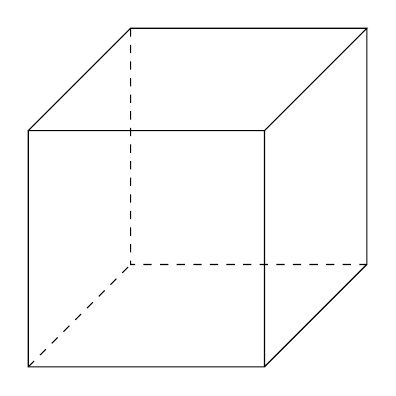
\begin{tikzpicture}
            \newcommand{\side}{3}
            \newcommand{\otherside}{1.3}
            \draw[dashed] (\otherside,\side+\otherside) -- (\otherside,\otherside) -- (\side+\otherside,\otherside)
            (0,0) -- (\otherside,\otherside);
            \draw (0,0) rectangle (\side,\side)
            (0,\side) -- (\otherside,\otherside+\side) -- (\otherside+\side,\otherside+\side) -- (\side,\side)
            (\otherside+\side,\otherside+\side) -- (\otherside+\side,\otherside) -- (\side,0);
\end{tikzpicture}
\end{center}

\subsection{Rectangular Prisms}

In this handout, a rectangular prism will always refer to a \textit{right} rectangular prism. Unless otherwise specified, rectangular prisms are right. This is generally true in competitions as well.

A non-right rectangular prism is a parallelepiped with a rectangular base.\footnote{See below for the definition of a parallelepiped.}

\begin{defi}[Right Rectangular Prism]
A rectangular prism is a solid with $6$ rectangular faces.
\end{defi}

\begin{theo}[Volume of a Right Rectangular Prism]
The volume of a rectangular prisms with side lengths $l,w,h$ is $lwh.$
\end{theo}

\begin{theo}[Surface Area of a Right Rectangular Prism]
The surface area of a rectangular prism with side lengths $l,w,h$ is $2(lw+wh+hl).$
\end{theo}

\begin{pro}
There are two faces with the dimensions $l\times w,$ $w\times h,$ and $h\times l.$ Multiplication and addition finish.
\end{pro}

\begin{center}
% \usetikzlibrary{positioning,calc}
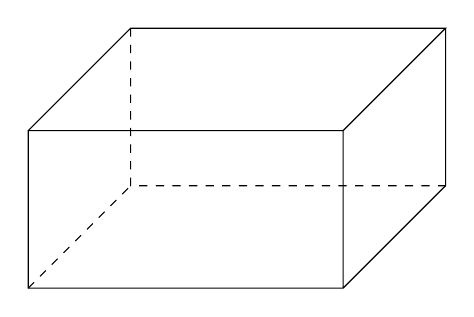
\begin{tikzpicture}
            \newcommand{\width}{3}
            \newcommand{\length}{4}
            \newcommand{\height}{2}
            \newcommand{\otherside}{1.3}
            \draw[dashed] (\otherside,\height+\otherside) -- (\otherside,\otherside) -- (\length+\otherside,\otherside)
            (0,0) -- (\otherside,\otherside);
            \draw (0,0) rectangle (\length,\height)
            (0,\height) -- (\otherside,\otherside+\height) -- (\otherside+\length,\otherside+\height) -- (\length,\height)
            (\otherside+\length,\otherside+\height) -- (\otherside+\length,\otherside) -- (\length,0);
\end{tikzpicture}
\end{center}

\begin{exam}
Three faces of a rectangular prism have areas $6,10,15.$ Find the volume of the rectangular prism.
\end{exam}
\begin{sol}
Let the side lengths be $a,b,c.$ Note that
\[ab=6\]
\[bc=10\]
\[ca=15,\]
and the volume of the prism is $abc.$ Multiplying all of the expressions together gives us $(abc)^2=900,$ or $abc=30.$
\end{sol}

\subsection{Exercises}


\begin{exer}
Consider a rectangular prism whose base has an area of $40$ and a height of $17.$ What is its volume?
\end{exer}
\begin{exer}
A right rectangular prism with a volume of $32000$ and a base width of $8$ and a base length of $10.$ When the prism is cut by a plane parallel and equidistant to both bases, what is the combined surface area of the two remaining figures?
\end{exer}

\subsection{General Parallelepipeds}

\begin{defi}[Parallelepipeds]
A parallelpiped is a solid with $6$ parallelogram faces.
\end{defi}
Note that all parallelepipeds are prisms.

\begin{theo}[Volume of a Parallelepiped]
The volume of a parallelepiped with a base of area $B$ and height $h$ is $Bh.$
\end{theo}

\begin{center}
    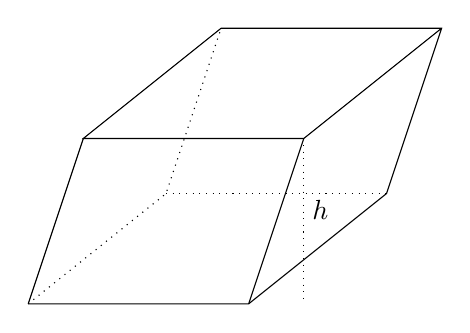
\begin{tikzpicture}[scale=0.7]
\draw (0,0) -- (4,0) -- (6.5,2) -- (7.5,5) -- (3.5,5) -- (1,3) -- (5,3) -- (7.5,5);
\draw (0,0) -- (1,3);
\draw (4,0) -- (5,3);
\draw [dotted] (0,0) -- (2.5,2) -- (3.5,5);
\draw [dotted] (2.5,2)--(6.5,2);
\draw [dotted] (5,3)--(5,0);
\node at (5.3,1.7) {$h$};
\end{tikzpicture}
\end{center}
The surface area of a parallelepiped should also not be too hard to compute.


\begin{exer}
A parallelelepiped has coordinates $(0,0,0),(2,0,0),(1,\sqrt{3},0),(3,\sqrt{3},0)$ for one face and coordinates $(1,0,2),(3,0,2),(2,\sqrt{3},2),(4,\sqrt{3},2)$ for the opposite face. Find its surface area.
\end{exer}


\section{Prisms and Cylinders}

\begin{defi}[Prism]
A prism is a solid with two congruent parallel faces, and the rest of its faces are parallelograms.
\end{defi}

\begin{theo}[Volume of a Prism]
The volume of a prism with a base of area $B$ and a height of $h$ is $Bh.$
\end{theo}
Note the similarity to the formula for the volume of a parallelpiped.

\begin{defi}[Cylinder]
A cylinder is a solid with two parallel circles as bases.
\end{defi}

\begin{theo}[Volume of a Cylinder]
The volume of a cylinder with a base if area $B$ and a height of $h$ is $Bh.$
\end{theo}
An alternative formulation of this is that the volume of a cylinder with radius $r$ and height $h$ is $\frac{\pi r^2h}{3}.$

\begin{defi}[Right and Oblique Cylinders]
A cylinder is right if the line joining the centers of its bases is perpendicular to the bases, and oblique otherwise.
\end{defi}
Unless otherwise specified, cylinders are right. This is generally true in competitions as well. Regardless, the volume formula \textit{always} holds.

\begin{center}
    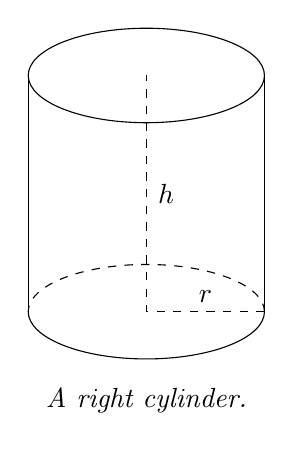
\begin{tikzpicture}
    \newcommand{\size}{1.5}
    \draw (-\size,0) arc (180:360:{\size} and 0.6);
    \draw[dashed] (\size,0) arc (0:180:{\size} and 0.6);
    \draw (-\size,\size+\size) arc (180:360:{\size} and 0.6);
    \draw (\size,\size+\size) arc (0:180:{\size} and 0.6);
    \draw (-\size,0)--(-\size,\size+\size);
    \draw (\size,0)--(\size,\size+\size);
    \draw[dashed] (\size,0)--(0,0)--(0,\size+\size);
    \node at (0,-\size+\size/4) {\textit{A right cylinder.}};
    %\filldraw (0,0) circle (1pt);
    \node at (\size/2,\size/8) {$r$};
    \node at (\size/6,\size) {$h$};
    \end{tikzpicture}
    \hspace{1.5cm}
    %\textit{A right cylinder.}
    %\\[1\baselineskip]
    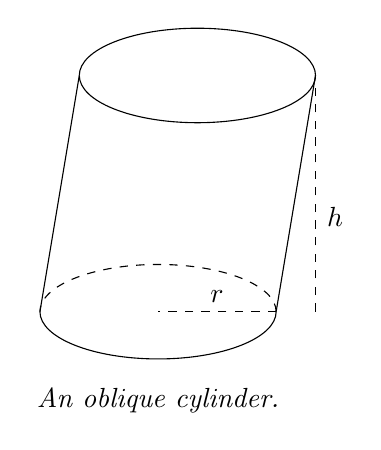
\begin{tikzpicture}
    \newcommand{\size}{1.5}
    \newcommand{\slant}{0.5}
    \draw (-\size,0) arc (180:360:{\size} and 0.6);
    \draw[dashed] (\size,0) arc (0:180:{\size} and 0.6);
    \draw (-\size+\slant,\size+\size) arc (180:360:{\size} and 0.6);
    \draw (\size+\slant,\size+\size) arc (0:180:{\size} and 0.6);
    \draw (-\size,0)--(-\size+\slant,\size+\size);
    \draw (\size,0)--(\size+\slant,\size+\size);
    \draw[dashed] (\size,0)--(0,0);
    \draw[dashed] (\size+\slant,0)--(\size+\slant,\size+\size);
    \node at (0,-\size+\size/4) {\textit{An oblique cylinder.}};
    %\filldraw (0,0) circle (1pt);
    \node at (\size/2,\size/8) {$r$};
    \node at (\slant+\size+\size/6,\size/5+\size/5+\size/5+\size/5) {$h$};
    \end{tikzpicture}
\end{center}

\begin{theo}[Surface Area of a Right Cylinder]
The surface area of a right cylinder with radius $r$ and height $h$ is $2\pi r^2+2\pi rh.$
\end{theo}

\begin{pro}
The two faces have area $\pi r^2$ each, and the circumference of the circle multiplied by the height gives $2\pi r\cdot h.$ Adding yields $2\pi r^2+2\pi rh.$
\end{pro}

\subsection{Exercises}


\begin{exer}
Consider a cylinder with diameter $10$ and height $7.$ What is its volume?
\end{exer}
\begin{exer}
Consider two right cylinders $P$ and $Q$ with the same volume. Cylinder $P$ has a radius $30\%$ longer than Cylinder $Q.$ What percent larger is the height of Cylinder $Q$ than that of Cylinder $P?$
\end{exer}


\section{Pyramids and Cones}

\subsection{Pyramids}
\begin{defi}[Pyramid]
A pyramid is a solid with a polygonal base whose vertices are all joined to a point not in the plane of the base. This point is called the \textit{apex}.
\end{defi}

The volume formula is identical to the volume of a cone.

\begin{theo}[Volume of a Pyramid]
The volume of a pyramid with a base of area $B$ and a height of $h$ is $\frac{Bh}{3}.$
\end{theo}

\subsection{Cones}
\begin{defi}[Cone]
A cone is a solid with a circular base where every point on the base is joined to a point not in the plane of the base. This point is called the \textit{apex}.
\end{defi}

The volume formula is identical to the volume of a pyramid.

\begin{theo}[Volume of a Cone]
The volume of a cone with a base of area $B$ and a height of $h$ is $\frac{Bh}{3}.$
\end{theo}
An alternative formulation of this is that the volume of a cone with radius $r$ and height $h$ is $\frac{\pi r^2h}{3}.$

\begin{defi}[Right and Oblique Cones]
A cone is right if the line joining the center of it bases with the apex is perpendicular to the base, and oblique otherwise.
\end{defi}
Unless otherwise specified, cones are right. This is generally true in competitions as well. Regardless, the volume formula \textit{always} holds.

\begin{center}
    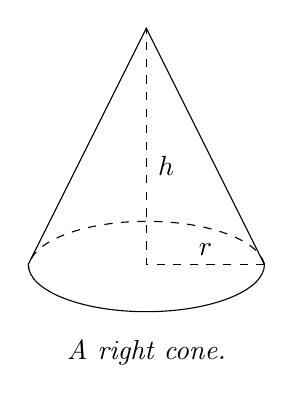
\begin{tikzpicture}
    \newcommand{\size}{1.5}
    \draw (-\size,0) arc (180:360:{\size} and 0.6);
    \draw[dashed] (\size,0) arc (5:180:{\size} and 0.6);
    
    \draw (-\size,0)--(0,\size+\size)--(\size,0);
    \draw[dashed] (\size,0)--(0,0)--(0,\size+\size);
    
    \node at (\size/2,\size/8) {$r$};
    \node at (\size/6,\size-\size/6) {$h$};
    
    \node at (0,-\size+\size/4) {\textit{A right cone.}};
    \end{tikzpicture}
    \hspace{1.5cm}
    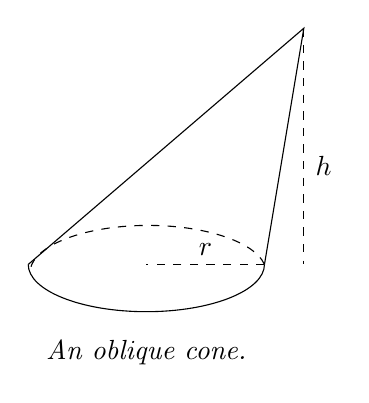
\begin{tikzpicture}
    \newcommand{\size}{1.5}
    \newcommand{\slant}{2}
    \draw (-\size,0) arc (180:360:{\size} and 0.6);
    \draw[dashed] (\size,0) arc (10:180:{\size} and 0.6);
    
    \draw (-\size,0)--(\slant,\size+\size)--(\size,0);
    \draw[dashed] (\size,0)--(0,0);
    \draw[dashed] (\slant,\size+\size)--(\slant,0);
    
    \node at (\size/2,\size/8) {$r$};
    \node at (\slant+\size/6,\size-\size/6) {$h$};
    
    \node at (0,-\size+\size/4) {\textit{An oblique cone.}};
    \end{tikzpicture}
\end{center}

\begin{theo}[Surface Area of a Right Cone]
The surface area of a cone with radius $r$ and height $h$ is $\pi r^2+2\pi r\sqrt{r^2+h^2}.$
\end{theo}

\begin{pro}
The area of the base is $\pi r^2,$ and the circumference multiplied by the slant height is $2\pi r\cdot \sqrt{r^2+h^2.}$ (Note that the slant height is $\sqrt{r^2+h^2}$ by the Pythagorean Theorem.) Adding gives $\pi r^2+2\pi r\sqrt{r^2+h^2}.$
\end{pro}

The surface area of an oblique cone is surprisingly hard to find.
\section{Spheres}
Spheres are the $3$ dimensional version of circles.
\begin{defi}[Sphere]
A sphere is the locus of points in space equidistant from a certain point. This point is called the center.
\end{defi}

\begin{theo}[Volume of a Sphere]
The volume of a sphere with radius $r$ is $\frac{4\pi r^3}{3}.$
\end{theo}

\begin{theo}[Surface Area of a Sphere]
The surface area of a sphere with radius $r$ is $4\pi r^2.$
\end{theo}

\begin{center}
    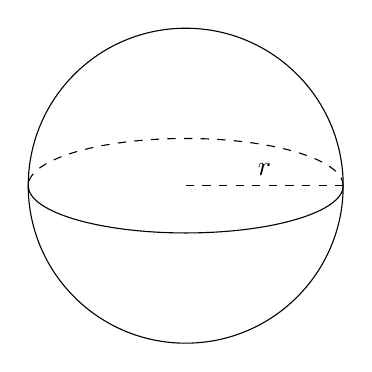
\begin{tikzpicture}
%  \shade[ball color = gray!40, opacity = 0.4] (0,0) circle (2cm);
  \draw (0,0) circle (2cm);
  \draw (-2,0) arc (180:360:2 and 0.6);
  \draw[dashed] (2,0) arc (0:180:2 and 0.6);
%  \fill[fill=black] (0,0) circle (1pt);
  \draw[dashed] (0,0 ) -- node[above]{$r$} (2,0);
\end{tikzpicture}
\end{center}


\begin{exer}
The numerical surface area and volume of a sphere are the same. What is the radius of this sphere?
\end{exer}


\begin{defi}[Cube]
A cube is a solid with $6$ square faces.
\end{defi}

\begin{theo}[Volume of a Cube]
The volume of a cube with side length $x$ is $x^3.$
\end{theo}

\begin{theo}[Surface Area of a Cube]
The surface area of a cube with side length $x$ is $6x^2.$
\end{theo}

\begin{pro}
There are six faces, and each face has area $x^2.$ Thus the total surface area is $6x^2.$
\end{pro}

\begin{center}
% \usetikzlibrary{positioning,calc}
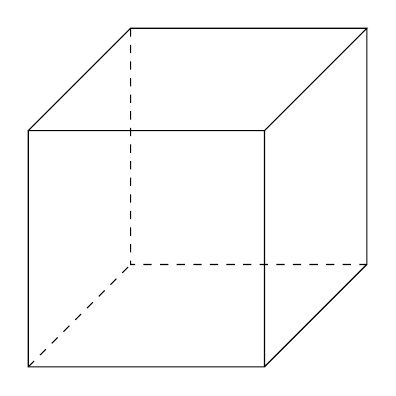
\begin{tikzpicture}
            \newcommand{\side}{3}
            \newcommand{\otherside}{1.3}
            \draw[dashed] (\otherside,\side+\otherside) -- (\otherside,\otherside) -- (\side+\otherside,\otherside)
            (0,0) -- (\otherside,\otherside);
            \draw (0,0) rectangle (\side,\side)
            (0,\side) -- (\otherside,\otherside+\side) -- (\otherside+\side,\otherside+\side) -- (\side,\side)
            (\otherside+\side,\otherside+\side) -- (\otherside+\side,\otherside) -- (\side,0);
\end{tikzpicture}
\end{center}

\subsection{Rectangular Prisms}

In this handout, a rectangular prism will always refer to a \textit{right} rectangular prism. Unless otherwise specified, rectangular prisms are right. This is generally true in competitions as well.

A non-right rectangular prism is a parallelepiped with a rectangular base.\footnote{See below for the definition of a parallelepiped.}

\begin{defi}[Right Rectangular Prism]
A rectangular prism is a solid with $6$ rectangular faces.
\end{defi}

\begin{theo}[Volume of a Right Rectangular Prism]
The volume of a rectangular prisms with side lengths $l,w,h$ is $lwh.$
\end{theo}

\begin{theo}[Surface Area of a Right Rectangular Prism]
The surface area of a rectangular prism with side lengths $l,w,h$ is $2(lw+wh+hl).$
\end{theo}

\begin{pro}
There are two faces with the dimensions $l\times w,$ $w\times h,$ and $h\times l.$ Multiplication and addition finish.
\end{pro}

\begin{center}
% \usetikzlibrary{positioning,calc}
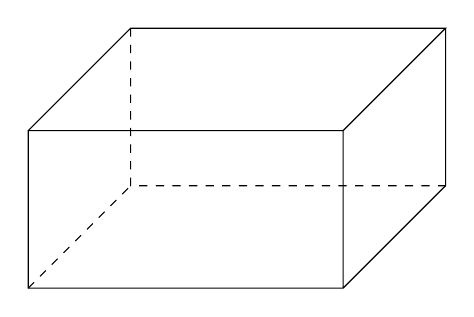
\begin{tikzpicture}
            \newcommand{\width}{3}
            \newcommand{\length}{4}
            \newcommand{\height}{2}
            \newcommand{\otherside}{1.3}
            \draw[dashed] (\otherside,\height+\otherside) -- (\otherside,\otherside) -- (\length+\otherside,\otherside)
            (0,0) -- (\otherside,\otherside);
            \draw (0,0) rectangle (\length,\height)
            (0,\height) -- (\otherside,\otherside+\height) -- (\otherside+\length,\otherside+\height) -- (\length,\height)
            (\otherside+\length,\otherside+\height) -- (\otherside+\length,\otherside) -- (\length,0);
\end{tikzpicture}
\end{center}

\begin{exam}
Three faces of a rectangular prism have areas $6,10,15.$ Find the volume of the rectangular prism.
\end{exam}
\begin{sol}
Let the side lengths be $a,b,c.$ Note that
\[ab=6\]
\[bc=10\]
\[ca=15,\]
and the volume of the prism is $abc.$ Multiplying all of the expressions together gives us $(abc)^2=900,$ or $abc=30.$
\end{sol}

\subsection{Exercises}


\begin{exer}
Consider a rectangular prism whose base has an area of $40$ and a height of $17.$ What is its volume?
\end{exer}
\begin{exer}
A right rectangular prism with a volume of $32000$ and a base width of $8$ and a base length of $10.$ When the prism is cut by a plane parallel and equidistant to both bases, what is the combined surface area of the two remaining figures?
\end{exer}


\section{Techniques}
We assume basic competence in 3D Geometry. This means knowing all of the volume and surface area formulas.

\subsection{Cross-sections}
Sometimes it's possible to simplify a problem into 2 dimensions. This makes it much easier to visualize. \textbf{Do this whenever possible.}

\begin{defi}[Cross-section]
A cross-section of a solid is the intersection of the solid with a plane.
\end{defi}

You can also take cross-sections of a cube and a cone. The former is used sometimes in math competitions, and the latter produces a shape known as a \textit{conic}.

\begin{theo}[Cross-section of a Cube]
The cross-section of a cube can be a triangle, quadrilateral, pentagon, or hexagon.
\end{theo}

The heuristical reason this is true is because a cube has $6$ faces, and the plane can intersect the cube at any $6$ of those faces. It's not too hard to construct any polygon with less than $7$ sides.

Sometimes the entire problem is reduced significantly or just solved by taking the correct cross section.

\begin{exam}
Inside a cone of radius $5$ and height $12$ there is a sphere inscribed. What is its radius?
\end{exam}
\begin{sol}
Here is a walkthrough of the solution.
\begin{enumerate}
    \item Take a cross section through the apex of the cone perpendicular to the base.
    
    \item Now you have a triangle and its incircle. Finish with $[ABC]=rs.$
\end{enumerate}
\end{sol}

\begin{exam}[AMC 10A 2019/21]
A sphere with center $O$ has radius 6. A triangle with sides of length $15$, $15$, and $24$ is situated in space so that each of its sides are tangent to the sphere. What is the distance between $O$ and the plane determined by the triangle?
\end{exam}
\begin{sol}
Here is a walkthrough of the solution.
\begin{enumerate}
    \item This is not actually a 3D geometry problem.

    \item Take a cross section of the sphere with the triangle.
    
    \item Use $[ABC]=rs$ to figure out the radius of the cross-section.
    
    \item Finish with the Pythagorean Theorem.
\end{enumerate}
\end{sol}

\subsection{Pythagorean Theorem}
Here are some demonstrations of assorted Pythagorean Theorem techniques.

\begin{exam}
Consider unit cube $ABCDEFGH,$ where $ABCD$ and $EFGH$ are opposite faces and $AG,$ $BH,$ $CE,$ $DF$ are space diagonals. Find the area of triangle $AFH.$
\end{exam}

\begin{sol}
Note that $AF=FH=HA=\sqrt{2}$ by the Pythagorean Theorem, so the area is $\frac{(\sqrt{2})^2\sqrt{3}}{4}=\frac{\sqrt{3}}{2}.$
\end{sol}

\begin{exam}[AHSME 1996/9]
Triangle $PAB$ and square $ABCD$ are in perpendicular planes. Given that $PA = 3, PB = 4$ and $AB = 5$, what is $PD?$

\begin{center}
    \begin{asy}
pen ExamColor = rgb(240,200,200);
size(5cm);
    import olympiad;
    real r=sqrt(2)/2;
draw(origin--(8,0)--(8,-1)--(0,-1)--cycle);
draw(origin--(8,0)--(8+r, r)--(r,r)--cycle);
filldraw(origin--(-6*r, -6*r)--(8-6*r, -6*r)--(8, 0)--cycle, ExamColor, black);
filldraw(origin--(8,0)--(8,6)--(0,6)--cycle, ExamColor, black);
pair A=(6,0), B=(2,0), C=(2,4), D=(6,4), P=B+1*dir(-65);
draw(A--P--B--C--D--cycle);
dot(A^^B^^C^^D^^P);
label("$A$", A, dir((4,2)--A));
label("$B$", B, dir((4,2)--B));
label("$C$", C, dir((4,2)--C));
label("$D$", D, dir((4,2)--D));
label("$P$", P, dir((4,2)--P));
    \end{asy}
\end{center}
\end{exam}

\begin{sol}
Note that $\angle PAD=90^{\circ},$ so $PD=\sqrt{PA^2+DA^2}=\sqrt{3^2+5^2}=\sqrt{34}.$
\end{sol}

For problems with tangent spheres, remember the following fact.
\begin{fact}[Tangency Point is Collinear with Centers]
If two spheres with centers $O_1,O_2$ are tangent at $T,$ then $O_1,O_2,T$ are collinear.
\end{fact}
This implies the following corollary.
\begin{fact}[Distance Between Centers]
Say two spheres $\Gamma_1,\Gamma_2$ with centers $O_1,O_2$ and radii $r_1,r_2$ are tangent at $T.$ Then
\[\begin{cases}
O_1O_2=r_1+r_2 \text{ if } \Gamma_2 \text{ is externally tangent to } \Gamma_1 \\
O_1O_2=r_1-r_2 \text{ if } \Gamma_2 \text{ is internally tangent to } \Gamma_1.
\end{cases}\]
\end{fact}
Using this in conjunction with the Pythagorean Theorem is enough to solve almost all problems with tangent spheres.
\begin{exam}[AMC 12A 2004/22]
Three mutually tangent spheres of radius $1$ rest on a horizontal plane. A sphere of radius $2$ rests on them. What is the distance from the plane to the top of the larger sphere?
\end{exam}
\begin{sol}
Let's label some points. Let the centers of the unit spheres be $O_1,O_2,O_3,$ let the center of the sphere of radius $2$ be $O,$ and let the foot of the perpendicular from $O$ to $O_1O_2O_3$ be $P.$ Note that $O_1O_2O_3$ is parallel to the horizontal plane with a distance of $1.$

Note that $\triangle O_1O_2O_3$ is equilateral with side length $2,$ and by symmetry, $P$ must be the center. Thus $PO_1=\frac{2\sqrt{3}}{3}.$ Since $OO_1=3$ by Fact $2,$ $OP=\sqrt{OO_1^2-PO_1^2}=\sqrt{3^2-(\frac{2\sqrt{3}}{3})^2}=\frac{\sqrt{69}}{3}.$

Since the distance from $P$ to the horizontal plane is $1$ and the tip of the sphere with radius $2$ is $2$ above $O,$ the answer is $1+2+\frac{\sqrt{69}}{3}=3+\frac{\sqrt{69}}{3}.$
\end{sol}
\begin{center}
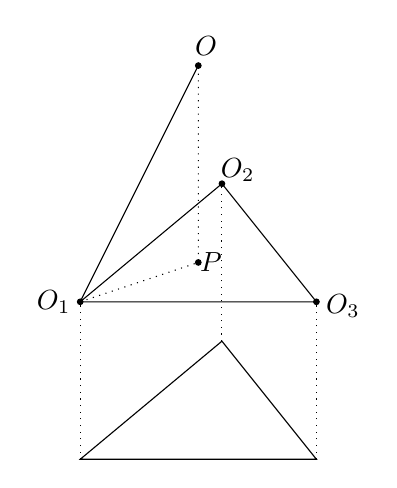
\begin{tikzpicture}
    \draw (0,0)--(1.8,1.5)--(3,0)--cycle;
    \draw (0,2)--(1.8,3.5)--(3,2)--cycle;
    \draw [dotted] (0,0)--(0,2);
    \draw [dotted] (1.8,1.5)--(1.8,3.5);
    \draw [dotted] (3,0)--(3,2);
    \draw [dotted] (0,2)--(1.5,2.5)--(1.5,5);
    \draw (1.5,5)--(0,2);
    \node at (0,2) [anchor=east] {$O_1$};
    \node at (2,3.4) [anchor=south] {$O_2$};
    \node at (3,1.95) [anchor=west] {$O_3$};
    \node at (1.4,2.5) [anchor=west] {$P$};
    \node at (1.6,5) [anchor=south] {$O$};
    \filldraw (0,2) circle (1pt);
    \filldraw (1.8,3.5) circle (1pt);
    \filldraw (3,2) circle (1pt);
    \filldraw (1.5,2.5) circle (1pt);
    \filldraw (1.5,5) circle (1pt);
\end{tikzpicture}
\end{center}

Notice that the entire solution was essentially just doing the correct setup and using the Pythagorean Theorem.

%\section{Tetrahedron Centers}

\pagebreak

\section{Problems}

\minpt{32}

\psetquote{Introducing change is like pulling off a bandage: the pain is a memory as soon as you feel it.}{Paul Graham}


\begin{prob}[]{1}
The net of a 3D figure is composed of 6 congruent squares and has a total area of 216 square inches. When the shape is folded to form a cube, how cubic inches are in its volume?
\end{prob}

\begin{center}
    \begin{asy}
    size(5cm);
    draw((0,0)--(4,0)--(4,1)--(0,1)--cycle);
    draw((1,-1)--(2,-1)--(2,2)--(1,2)--cycle);
    draw((3,0)--(3,1));
    \end{asy}
\end{center}

\begin{prob}[AMC 12A 2008/8]{1}
What is the volume of a cube whose surface area is twice that of a cube with volume 1?
\end{prob}

\begin{prob}[AMC 12B 2005/16]{2}
Eight spheres of radius 1, one per octant, are each tangent to the coordinate planes. What is the radius of the smallest sphere, centered at the origin, that contains these eight spheres?
\end{prob}

\begin{prob}[]{2}
A pyramid has a square base $ABCD$ and vertex $E$. The area of square $ABCD$ is $196$, and the areas of $\triangle ABE$ and $\triangle CDE$ are $105$ and $91$, respectively. What is the volume of the pyramid?
\end{prob}

\begin{prob}[]{2}
Consider two externally tangent spheres $\Gamma_1$ and $\Gamma_2$ with radii $12,r,$ and consider cylinder $\Omega$ with radius $16$ and height $25.$ If $\Gamma_1$ is internally tangent to a base and the circumference of $\Omega$ and $\Gamma_2$ is internally tangent to the opposite base and the circumference of $\Omega,$ find $r.$
\end{prob}

\begin{req}[AMC 10B 2018/10]{2}
In the rectangular parallelepiped shown, $AB$ = $3$, $BC$ = $1$, and $CG$ = $2$. Point $M$ is the midpoint of $\overline{FG}$. What is the volume of the rectangular pyramid with base $BCHE$ and apex $M$?
\end{req}

\begin{center}
    \begin{asy}
    import olympiad;
    size(6cm);
pair A = origin;
pair B = (4.75,0);
pair E1=(0,3);
pair F = (4.75,3);
pair G = (5.95,4.2);
pair C = (5.95,1.2);
pair D = (1.2,1.2);
pair H= (1.2,4.2);
pair M = ((4.75+5.95)/2,3.6);
draw(E1--M--H--E1--A--B--E1--F--B--M--C--G--H);
draw(B--C);
draw(F--G);
draw(A--D--H--C--D,dashed);
label("$A$",A,SW);
label("$B$",B,SE);
label("$C$",C,E);
label("$D$",D,W);
label("$E$",E1,W);
label("$F$",F,SW);
label("$G$",G,NE);
label("$H$",H,NW);
label("$M$",M,N);
dot(A);
dot(B);
dot(E1);
dot(F);
dot(G);
dot(C);
dot(D);
dot(H);
dot(M);
label("3",A/2+B/2,S);
label("2",C/2+G/2,E);
label("1",C/2+B/2,SE);
    \end{asy}
\end{center}

\begin{prob}[AIME 1984/9]{2}
In tetrahedron $ABCD$, edge $AB$ has length 3 cm. The area of face $ABC$ is $15\mbox{cm}^2$ and the area of face $ABD$ is $12 \mbox { cm}^2$. These two faces meet each other at a $30^\circ$ angle. Find the volume of the tetrahedron in $\mbox{cm}^3$.
\end{prob}

\begin{prob}[AMC 12B 2008/18]{2}
On a sphere with a radius of $2$ units, the points $A$ and $B$ are $2$ units away from each other. Compute the distance from the center of the sphere to the line segment $AB.$
\end{prob}

\begin{prob}[AMC 10A 2013/22]{3}
Six spheres of radius $1$ are positioned so that their centers are at the vertices of a regular hexagon of side length $2$. The six spheres are internally tangent to a larger sphere whose center is the center of the hexagon. An eighth sphere is externally tangent to the six smaller spheres and internally tangent to the larger sphere. What is the radius of this eighth sphere?
\end{prob}

\begin{prob}[AMC 12A 2005/22]{3}
A rectangular box $P$ is inscribed in a sphere of radius $r$. The surface area of $P$ is 384, and the sum of the lengths of its 12 edges is 112. What is $r$?
\end{prob}

\begin{prob}[AIME I 2020/6]{3}
A flat board has a circular hole with radius $1$ and a circular hole with radius $2$ such that the distance between the centers of the two holes is $7.$ Two spheres with equal radii sit in the two holes such that the spheres are tangent to each other. The square of the radius of the spheres is $\tfrac{m}{n},$ where $m$ and $n$ are relatively prime positive integers. Find $m+n.$
\end{prob}

\begin{prob}[AMC 12B 2004/19]{3}
A truncated cone has horizontal bases with radii $18$ and $2$. A sphere is tangent to the top, bottom, and lateral surface of the truncated cone. What is the radius of the sphere?
\end{prob}

\begin{prob}[AIME II 2020/7]{4}
Two congruent right circular cones each with base radius $3$ and height $8$ have axes of symmetry that intersect at right angles at a point in the interior of the cones a distance $3$ from the base of each cone. A sphere with radius $r$ lies inside both cones. The maximum possible value for $r^2$ is $\frac mn$, where $m$ and $n$ are relatively prime positive integers. Find $m+n$.
\end{prob}

\begin{prob}[AHSME 1996/28]{4}
On a $4\times 4\times 3$ rectangular parallelepiped, vertices $A$, $B$, and $C$ are adjacent to vertex $D$. Find the distance from $D$ to plane $ABC$.
\end{prob}


\begin{prob}[AIME I 2001/12]{6}
A sphere is inscribed in the tetrahedron whose vertices are $A = (6,0,0), B = (0,4,0), C = (0,0,2),$ and $D = (0,0,0).$ The radius of the sphere is $m/n,$ where $m$ and $n$ are relatively prime positive integers. Find $m + n.$
\end{prob}

\begin{prob}[AIME I 2013/7]{6}
A rectangular box has width $12$ inches, length $16$ inches, and height $\frac{m}{n}$ inches, where $m$ and $n$ are relatively prime positive integers. Three faces of the box meet at a corner of the box. The center points of those three faces are the vertices of a triangle with an area of $30$ square inches. Find $m+n$.
\end{prob}

\begin{req}[NARML 10]{9}
Three mutually tangent spheres with radii of $1$ are tangent to a table, and a cone is tangent to all three spheres with its tip oriented towards the table. If the cone has height $\sqrt{2}$ and its tip is $\tfrac{3+\sqrt{3}}{3}$ units above the table, compute the radius of the cone.
\end{req}

\begin{prob}[AIME II 2020/7]{9}
Two congruent right circular cones each with base radius $3$ and height $8$ have axes of symmetry that intersect at right angles at a point in the interior of the cones a distance $3$ from the base of each cone. A sphere with radius $r$ lies inside both cones. The maximum possible value for $r^2$ is $\frac mn$, where $m$ and $n$ are relatively prime positive integers. Find $m+n$.
\end{prob}


\begin{prob}[AIME II 2016/14]{13}
Equilateral $\triangle ABC$ has side length $600$. Points $P$ and $Q$ lie outside the plane of $\triangle ABC$ and are on opposite sides of the plane. Furthermore, $PA=PB=PC$, and $QA=QB=QC$, and the planes of $\triangle PAB$ and $\triangle QAB$ form a $120^{\circ}$ dihedral angle (the angle between the two planes). There is a point $O$ whose distance from each of $A,B,C,P,$ and $Q$ is $d$. Find $d$.
\end{prob}

\begin{prob}[AIME II 2017/15]{13}
Tetrahedron $ABCD$ has $AD=BC=28$, $AC=BD=44$, and $AB=CD=52$. For any point $X$ in space, define $f(X)=AX+BX+CX+DX$. The least possible value of $f(X)$ can be expressed as $m\sqrt{n}$, where $m$ and $n$ are positive integers, and $n$ is not divisible by the square of any prime. Find $m+n$.
\end{prob}
\end{document}